\part{基本服务篇}

本章介绍几种常见的服务。这里不注重概念的介绍,概念只做简短的描述,主要
介绍如何实施及实现这些服务。

\chapter{DHCP}

随着网络规模的不断扩大和网络复杂度的提高,计算机的数量经常超过可分配
的IP地址数量。同时随着便携机及无线网络的广泛使用,计算机的位置也经常变
化,相应的IP地址也必须经常更新,从而导致网络配置越来越复
杂。DHCP(Dynamic Host Configuration Protocol,动态主机配置协议)就是为
满足这些需求而发展起来的。

DHCP提供安全、可靠且简单的TCP/IP网络设置,避免了TCP/IP网络中地址的冲突,
同时也降低了管理IP地址设置的工作强度。使用DHCP主要的好处有以下几点:

\begin{enumerate}[itemsep=0pt,parsep=0pt]
\item 减少管理员的工作量
\item 减小输入错误的可能
\item 避免IP冲突
\item 当罗更改IP地址段时,不需要重新配置每台计算机的IP
\item 计算机移动不必重新配置TCP/IP信息
\item 提高了IP地址的利用率
\end{enumerate}

当一台DHCP客户端启动时,该客户端将在网络中请求IP地址,当DHCP服务器收到
申请IP地址请求后,它将从可用的地址中选择一个提供给DHCP客户端。

客户端除了可以从DHCP服务器得到IP地址信息外,还可以得到子网掩码、默认网
关、DNS服务器等其他TCP/IP信息。一般这些信息并非永久使用,而是有一个使用
的期限,这个期限被称为租约。所以DHCP服务器与客户端之间的通信分为两类,
即租约产生及租约更新。

DHCP的作用是为局域网中的每台计算机自动分配TCP/IP信息,包括IP地址、子网
掩码、网关以及DNS服务器等。其优点是终端无须配置,且网络维护方便。

动态主机配置协议(DHCP)\index{DHCP},

\begin{enumerate}[itemsep=0pt,parsep=0pt]
\item 服务端端口67/UDP
\item 客户端端口68/UDP
\item 客户端发送DHCPDISCOVER在网络中寻求地址分配
\item 服务端回应DHCPDISCOVER请求
\item 客户端发送DHCPREQUEST
\item 服务端发送DHCPACK
\item 客户端得到地址
\end{enumerate}

主配 cp /usr/share/doc/dhcp-<version>/dhcpd.conf.sample /etc/dhcpd.conf
包含以下7项 服务器即可搭建

\small{
\begin{verbatim}
1. ddns-update-style
2. subnet
3. option
4. range dynamic-bootp
5. default-lease-time
6. max-lease-time
7. host
\end{verbatim}
}
\normalsize

\small{
\begin{verbatim}
ddns-update-style interim;
ignore client-updates;
default-lease-time 600;
max-lease-time 7200;

subnet 192.168.0.0 netmask 255.255.255.0 {
    next-server 192.168.0.128;
    filename="pxelinux.0";
    option routers 192.168.0.128;
    option subnet-mask 255.255.255.0;
    option nis-domain "lavenliu.com";
    option domain-name "lavenliu.com";
    option ntp-servers 192.168.0.254;
    range dynamic-bootp 192.168.0.100 192.168.0.130;
    host stu1 {
      next-server lavenliu.com;
      hardware Ethernet 12:34:56:78:AB:CD;
      fixed-address 192.168.0.2;
    }
}
\end{verbatim}
}
\normalsize

%%% Local Variables:
%%% mode: latex
%%% TeX-master: t
%%% End:


\chapter{DNS}
\label{chap:dns}

在TCP/IP网络中,IP地址是网络节点的标识。但是,IP地址是点分十进制数字,
难以记忆。联想到在现实生活中,名字比身份证号码更容易被人记住,那么是否
可以拿名字来标识某个网络节点呢?答案是肯定的。DNS(Domain Name System,
域名系统)是一种用于TCP/IP应用程序的分布式数据库,提供域名与IP地址之间
的转换。

\section{测试环境}
\label{sec:dnsTestEnv}

以下测试是在CentOS6U5 64位系统上进行测试。系统均关闭iptables及selinux,
如果要开启iptables,请设置允许开放本机的53端口。

\begin{table}[htbp]
  \centering
    \caption{DNS演示环境机器一览}
    \label{tab:dnsMachines}
    \begin{tabular}{llr}
      \toprule
      主机名     & IP地址 & 说明 \\
      \midrule
      master01.lavenliu.com  & 192.168.20.134 &  主DNS \\
      minion01.lavenliu.com  & 192.168.20.135 &  辅DNS \\
      minion02.lavenliu.com  & 192.168.20.136 &  客户端 \\
      \bottomrule
    \end{tabular}
\end{table}

\section{安装及配置主DNS}
\label{sec:configMasterDNS}

在master01.lavenliu.com上安装如下软件包,

\begin{verbatim}
[root@master01 ~]# yum install -y bind bind-utils
\end{verbatim}

接下来配置主DNS,有两个文件需要修改,一个是主配置文件/etc/named.conf及/etc/named.rfc1912.zones文件。
首先配置/etc/named.conf文件,配置内容如下,在options字段中做如下修改:

\begin{verbatim}
listen-on port 53 { 127.0.0.1; 192.168.20.134; }; // 192.168.20.134 is Master DNS Server IP
listen-on-v6 port 53 { ::1; };
directory	"/var/named";
dump-file	"/var/named/data/cache_dump.db";
	statistics-file "/var/named/data/named_stats.txt";
	memstatistics-file "/var/named/data/named_mem_stats.txt";
allow-query		{ localhost; 192.168.20.0/24; }; // IP range
allow-transfer	{ localhost; 192.168.20.135; }; // 192.168.20.135 is Slave DNS Server IP
\end{verbatim}

接下来修改/etc/named.rfc1912.zones文件,在该文件末尾追加如下内容:

\begin{verbatim}
cat >> /etc/named.rfc1912.zones <<EOF
zone "lavenliu.com" IN {
     type master;
     file "forward.lavenliu";
     allow-update { none; };
};

zone "20.168.192.in-addr.arpa" IN {
     type master;
     file "reverse.lavenliu";
     allow-update { none; };
};
EOF
\end{verbatim}

由于我们在/etc/named.rfc1912.zones文件中设置了两个区域文件,分别为forward.lavenliu及reverse.lavenliu两个区域文件。
这两个文件分别是正向解析文件与反向解析文件,接下来就创建两个文件,这两个文件的位置默认是/var/named目录下。

首先,创建正向解析文件,

\begin{verbatim}
# vi /var/named/forward.lavenliu
$TTL 86400
@   IN  SOA     master01.lavenliu.com. root.lavenliu.com. (
		        2016051201  ;Serial
				3600        ;Refresh
				1800        ;Retry
				604800      ;Expire
				86400       ;Minimum TTL
)
@           IN  NS          master01.lavenliu.com.
@           IN  NS          minion01.lavenliu.com.
@           IN  A           192.168.20.134
@           IN  A           192.168.20.135
@           IN  A           192.168.20.136
master01    IN  A   	    192.168.20.134
minion01    IN  A   	    192.168.20.135
minion02    IN  A   	    192.168.20.136
\end{verbatim}

其次,创建反向解析文件,

\begin{verbatim}
# vi /var/named/reverse.lavenliu
$TTL 86400
@   IN  SOA     master01.lavenliu.com. root.lavenliu.com. (
		        2016051201  ;Serial
				3600        ;Refresh
				1800        ;Retry
				604800      ;Expire
				86400       ;Minimum TTL
)
@           IN  NS      master01.lavenliu.com.
@           IN  NS      minion01.lavenliu.com.
@           IN  PTR     lavenliu.com.
master01    IN  A   	192.168.20.134
minion01    IN  A   	192.168.20.135
minion02    IN  A   	192.168.20.136
134	    IN	PTR	master01.lavenliu.com.
135	    IN	PTR	minion01.lavenliu.com.
136	    IN	PTR	minion02.lavenliu.com.
\end{verbatim}

\subsection{启动DNS服务}
\label{sec:startDNS}

有了以上步骤的配置,我们就可以启动主DNS了。在启动之前,最好检查一下我们的配置文件的语法是否正确,
另外一个就是文件的权限问题了。由于我们是用root用户创建的正向及反向解析文件,
所以这两个文件的所有者及所属组均为root用户和组,接下来的第一件事情就是修改这两个文件的权限,

\begin{verbatim}
[root@master01 named]# chown -R named.named /var/named
[root@master01 named]# ll /var/named/
total 36
drwxrwx--- 2 named named 4096 Mar 16 21:25 data
drwxrwx--- 2 named named 4096 Mar 16 21:25 dynamic
-rw-r--r-- 1 named named  531 May 14 21:54 forward.lavenliu
-rw-r----- 1 named named 2075 Apr 23  2014 named.ca
-rw-r----- 1 named named  152 Dec 15  2009 named.empty
-rw-r----- 1 named named  152 Jun 21  2007 named.localhost
-rw-r----- 1 named named  168 Dec 15  2009 named.loopback
-rw-r--r-- 1 named named  564 May 14 21:57 reverse.lavenliu
drwxrwx--- 2 named named 4096 Mar 16 21:25 slaves
\end{verbatim}

接下来检查正向及反向解析文件的语法正确性,

\begin{verbatim}
[root@master01 ~]# named-checkconf /etc/named.conf
[root@master01 ~]# named-checkzone lavenliu.com /var/named/forward.lavenliu
zone lavenliu.com/IN: loaded serial 2016051201
OK
[root@master01 ~]# named-checkzone lavenliu.com /var/named/reverse.lavenliu
zone lavenliu.com/IN: loaded serial 2016051201
OK
\end{verbatim}

看上去没有问题,接下来就可以启动named服务了,
\begin{verbatim}
[root@master01 ~]# /etc/init.d/named start 
\end{verbatim}

启动之后,最好检查一下named的进程是否启动成功及53端口是否监听,

\begin{verbatim}
ps -ef |grep named |grep -v grep
netstat -antup |grep named |grep -v grep
\end{verbatim}

%%% Local Variables:
%%% mode: latex
%%% TeX-master: t
%%% End:


\chapter{FTP}
\label{chap:FTP}

在互联网中,人们经常需要在远端主机与本地服务器之间传输文件,文件传输协
议提供的应用服务满足了人们的这种需求。FTP(File Transfer Protocol,文件
传输协议)是互联网上文件传输的标准协议,FTP使用TCP作为传输协议,支持用
户的登录认证及访问权限的设置。互联网上另一种常用的文件传输协议
是TFTP(Trivial File Transfer Protocol,普通文件传输协议),TFTP是一种
简单的文件传输协议,不支持用户的登录认证,也不具备复杂的命
令。TFTP使用UDP作为传输协议,并具有重传机制。

%%% Local Variables:
%%% mode: latex
%%% TeX-master: t
%%% End:


\chapter{NFS}
\label{chap:NFS}

NFS(Network File System)\index{NFS}网络文件系统,目前依然非常流行。
NFS的一个最大优点是具有广泛的支持:大部分的类UNIX都可以支持NFS。NFS通常
比其他的网络文件系统更容易配置和使用。与其他网络文件系统一样,NFS可以在
服务器或任何一个客户端上修改文件,然后在其他所有系统上可以立即使用修改
后的文件。

安装很简单:

\section{配置NFS服务器}

\section{配置NFS客户端}

客户端基本上不用配置就可以使用。

%%% Local Variables:
%%% mode: latex
%%% TeX-master: t
%%% End:


\chapter{Kickstart}

Red Hat Linux提供了一种非常方便的自动化系统安装方式,即为
kickstart\index{kickstart}。这种工具的出现,极大的方便了众多的系统管理
员或装机攻城狮。有了它,我们就不用拿着光盘或U盘在机房来回乱窜地装机了,
我们可以在办公室通过IPMI的方式来操作。不管这个工具有多优秀,相比之前单
台的安装方式,效率提升了很多。当然,也有另外几种较优越的自动化系统安装
工具,这里就不介绍了。

kickstart文件包含了安装程序所使用的指令,在安装的过程中可以用来减少或者
消除用户输入的麻烦。

在系统数目巨大且完全相同的时候,kickstart文件非常有用。


\begin{figure}[htbp]
  \begin{center}
    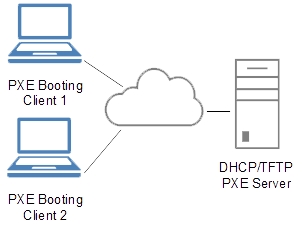
\includegraphics[width=.5\textwidth]{img/PXE_diagram.png}
  \end{center}
  \caption{PXE WorkFlow}
  \label{fig:pxeWork}
\end{figure}

PXE工作流程图:
\begin{figure}[htbp]
  \begin{center}
    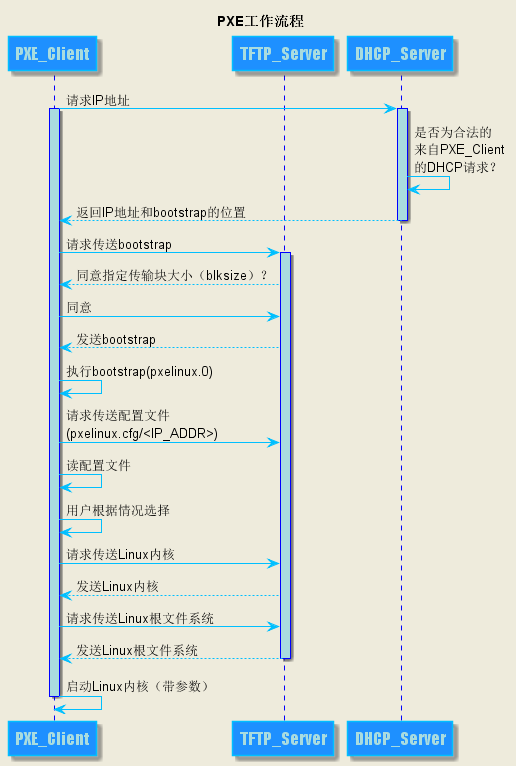
\includegraphics[width=.55\textwidth]{img/pxe01.png}
  \end{center}
  \caption{PXE工作流程图}
  \label{fig:pxeWorkFlow}
\end{figure}

\subsection{安装相关软件包}

\small{
\begin{verbatim}
	rpm -ivh dhcpdxxx
	rpm -ivh nfs-utilsxxx
	rpm -ivh tftp-serverxxx
	rpm -ivh xinetdxxx
	rpm -ivh httpdxxx
	rpm -ivh syslinuxxxx
	rpm -ivh system-config-kickstartxxx
\end{verbatim}
}
\normalsize

\small{
\begin{verbatim}
 # chkconfig tftp on
   # chkconfig xinetd on
\end{verbatim}
}
\normalsize
   
3. Stop some services, such as selinux, iptables
   setenforce 0
or  vi /etc/sysconfig/selinux disabled
    service iptables stop

4. Copy the related files to the related path

\small{
\begin{verbatim}
# mount /dev/cdrom /media
# mkdir /var/ftp/pub/RedHat
# cp -a /media/* /var/ftp/pub/RedHat
# cp /usr/share/syslinux/pxelinux.0 /tftpboot
# cp /var/ftp/pub/RedHat/isolinux/vmlinuz /tftpboot
# cp /var/ftp/pub/RedHat/isolinux/initrd.img /tftpboot
# mkdir /tftpboot/pxelinux.cfg
# vi /tftpboot/pxelinux.cfg/default 
     default install
     prompt 1
     timeout 60
     label local
	localhost	1
     label install
	kernel vmlinuz
	append initrd=initrd.img ramdisk_size=8192 ks=http://192.168.0.254/ks/ks.conf
\end{verbatim}
}
\normalsize

\small{
\begin{verbatim}
   # mount /dev/cdrom /media
   # mkdir /var/ftp/pub/RedHat
   # cp -a /media/* /var/ftp/pub/CentOS
   # cp /usr/share/syslinux/pxelinux.0 /var/lib/tftpboot
   # cp /var/ftp/pub/CentOS/isolinux/vmlinuz /var/lib/tftpboot
   # cp /var/ftp/pub/CentOS/isolinux/initrd.img /var/lib/tftpboot
   # mkdir /var/lib/tftpboot/pxelinux.cfg
   # vi /var/lib/tftpboot/pxelinux.cfg/default
	default install
	prompt 1
	timeout 60
	label local
		localhost	1
	label install
		kernel vmlinuz
		append initrd=initrd.img ramdisk_size=8192 ks=http://192.168.0.254/ks/ks.conf
\end{verbatim}
}
\normalsize

5. Modify the related configure files

\small{
\begin{verbatim}
# vi /etc/dhcp/dhcpd.conf
......
......
next-server	ip_addr;
filename	"pxelinux.0";
......

# vi /etc/http/conf/httpd.conf
Allow from all
# chown -R apache.apache /var/www

# vi /etc/exports
/var/ftp/pub/RedHat 192.168.0.0/255.255.255.0(ro,sync)
\end{verbatim}
}
\normalsize

6. Start services, and later the client can install OS

\small{
\begin{verbatim}
   # service xinetd restart
   # service nfs restart
   # service vsftpd restart
   # service httpd restart
   # service dhcpd restart
\end{verbatim}
}
\normalsize

\begin{verbatim}
NOTE:
In the ks.cfg, the keyword 
clearpart --none is default
change this into:
clearpart --all
\end{verbatim}

%%% Local Variables:
%%% mode: latex
%%% TeX-master: t
%%% End:


\chapter{Samba}

\chapter{Apache}
\label{chap:apache}

Apache HTTP Server是Apache软件基金会的一个开源Web服务器,可以在大多数操
作系统中运行,由于其多平台和安全性被广泛使用,是最流行的Web服务器软件之
一。

Apache支持许多特性,而这些特性大部分通过编译的模块实现。这些特性从服务
器端的编程语言支持到身份认证方案等包括目前所有流行的Web服务器应用。由
于Apache良好的开放性,目前也有很多非官方的模块用以满足某些特殊的应用,
在Apache 2.x中默认包含的模块如表所示:

\section{安装及配置Apache}
\label{subsec:InstallApache}

%%% Local Variables:
%%% mode: latex
%%% TeX-master: t
%%% End:


\chapter{Nginx}
\label{chap:nginx}

\section{关于Nginx}
\label{subsec:AboutNginx}

Nginx是由俄罗斯人Igor Sysoev为俄罗斯访问量第二Rambler.ru站
点开发的,它已经在该站点运行超过两年半了。它的发音为“engine
X”, 是一个高性能的HTTP和反向代理服务器,同时也是一个IMAP/POP3/SMTP 代
理服务器。Igor Sysoev在建立的项目时,使
用基于BSD许可。自Nginx发布四年来,Nginx已经因为它的稳定性、丰富的功能
集、示例配置文件和低系统资源的消耗而闻名。

在俄罗斯许多大网站都已经使用它,且一直表现不凡。截至2007年4月,俄罗斯
大约有20\%左右的虚拟主机是由Nignx服务或代理的。Google在线安全博客中统
计Nginx服务或代理了大约所有Internet虚拟主机的4\%。而Netcraft的统计显
示,Nginx服务的主机在过去的一年里以四倍的速度增长并且在这几年里,它的排
名还在不断上升,下图为Netcraft截止至2010年5月的统计。

\section{Nginx的安装与启动}
\label{subsec:InstallAndStartNginx}

Linux下安装软件有三种方式,这里我以源代码编译安装为主。服务器最小化安装
后,安装依赖包。

\begin{verbatim}
yum install -y pcre-devel \
gcc \
zlib-devel \
openssl-devel
\end{verbatim}

出于管理和安全的目的,我们希望使用一个指定的普通用户身份去运行我们的
Web服务器。所以,我们首先增加一个普通用户用于运行我们的Nginx。

\begin{verbatim}
groupadd nginx
useradd -g nginx nginx
\end{verbatim}

\begin{verbatim}
service iptables stop
chkconfig iptables off
\end{verbatim}

然后下载、解压并编译安装我们的Nginx,

\begin{verbatim}
wget http://nginx.org/download/nginx-1.8.0.tar.gz
tar -xf nginx-1.8.0.tar.gz -C /usr/local/src
cd /usr/local/src/nginx-1.8.0
./configure --user=nginx \
> --group=nginx \
> --with-http_ssl_module \
> --with-http_sub_module
\end{verbatim}

安装过程比较简单,./configure过程会报出一些依赖关系,这里已经解决。下面
来看看./configure后面几个常用的参数:

\begin{verbatim}
--prefix=<dir>         指定安装主目录,默认为/usr/local/nginx
--user=<user>          指定用户身份,如果没有指定则默认使用nobody
--group=<group>        指定组身份
--with-http_ssl_module 启用https支持
\end{verbatim}

\section{Nginx的基本配置}
\label{subsec:NginxConf}

Linux下基本上每个服务都会有它的主配置文件,该文件会定义服务应该如果去运
行,使用些什么参数,启用些什么功能,相关会涉及到的一些操作文件在哪,所
以主配置文件对服务是至关重要的。下面我们来分析一下Nginx的主配置文件。

\subsection{Nginx主配置概述}

Linux下基本上每个服务都会有它的主配置文件,该文件会定义服务应该如果去运
行,使用些什么参数,启用些什么功能,相关会涉及到的一些操作文件在哪,所以主
配置文件对服务是至关重要的。Nginx的主配置文件默认情况下位于
/usr/local/nginx/conf/nginx.conf,以下为Nginx配置文件一些参数的注释。

\begin{verbatim}
#user nobody;
#指定使用的用户
worker_processes 1;
#开启的进程数,一般设置 1-5
#error_log logs/error.log;
#error_log logs/error.log notice;
#error_log logs/error.log info;
#定义错误日志,以及记录的日志等级
#pid
logs/nginx.pid;
#定义 pid 文件位置
events {
# use [ kqueue | rtsig | epoll | /dev/poll | select | poll ];
#use epoll; #使用 epoll(linux2.6 的高性能方式)
#Nginx 支持如下处理连接的方法(I/O 复用方法),这些方法可以通过 use 指令指定。
#select - 标准方法。 如果当前平台没有更有效的方法,它是编译时默认的方法。你可以使用配置参
数 –with-select_module 和 –without-select_module 来启用或禁用这个模块。
#poll - 标准方法。 如果当前平台没有更有效的方法,它是编译时默认的方法。你可以使用配置参数
–with-poll_module 和 –without-poll_module 来启用或禁用这个模块。
#kqueue - 高效的方法,使用于 FreeBSD 4.1+, OpenBSD 2.9+, NetBSD 2.0 和 MacOS X. 使用双
处理器的 MacOS X 系统使用 kqueue 可能会造成内核崩溃。
#epoll - 高效的方法,使用于 Linux 内核 2.6 版本及以后的系统。在某些发行版本中,如 SuSE 8.2,
有让 2.4 版本的内核支持 epoll 的补丁。
#rtsig - 可执行的实时信号,使用于 Linux 内核版本 2.2.19 以后的系统。可是从 Linux 内核版本
2.6.6-mm2 开始,这个参数就不再使用了.
#/dev/poll - 高效的方法,使用于 Solaris 7 11/99+, HP/UX 11.22+ (eventport), IRIX 6.5.15+ 和
Tru64 UNIX 5.1A+.
#eventport - 高效的方法,使用于 Solaris 10. 为了防止出现内核崩溃的问题, 有必要安装这个安全补丁。
worker_connections 1024;
#worker_connections 51200; #每个进程最大连接数(最大连接=连接数 x 进程数)
}
http {
include
mime.types;
#文件扩展名与文件类型映射表
default_type application/octet-stream;
#默认文件类型
#log_format main '$remote_addr - $remote_user [$time_local] "$request" '
# '$status $body_bytes_sent "$http_referer" '
# '"$http_user_agent" "$http_x_forwarded_for"';
#access_log logs/access.log main;
sendfile
on;
#开启高效文件传输模式
#tcp_nopush
on;
#该选项用于防止网络阻塞
#keepalive_timeout 0;
keepalive_timeout 65;
##长链接超时时间
#gzip on;
#打开 gzip 压缩
#fastcgi_connect_timeout 300;
#fastcgi_send_timeout 300;
#fastcgi_read_timeout 300;
#fastcgi_buffer_size 128k;
#fastcgi_buffers 4 256k;
#fastcgi_busy_buffers_size 256k;
#fastcgi_temp_file_write_size 256k;
#fastcgi_temp_path /dev/shm;
#fastcgi 连接超时时间和缓存
server {
listen
80;
server_name localhost;
#主机名
#charset koi8-r;
#默认字符编码 charset gb2312
#access_log logs/host.access.log main;
location / {
#pass 路径匹配 能够匹配路径中带“/”的 不过需要注意的是如果之后也有相关“/”匹配项并且
使用比此处更精确匹配符,则以之后表达式优先
root html;
index index.html index.htm;
}
#error_page 404
/404.html;
# redirect server error pages to the static page /50x.html
#
error_page 500 502 503 504 /50x.html;
location = /50x.html {
#精确的匹配,并且不再向下匹配
root html;
}
#
#location ~ \.php$ {
#正则表达式匹配 一旦匹配则不再向下匹配
#
proxy_pass http://127.0.0.1;
#}
# pass the PHP scripts to FastCGI server listening on 127.0.0.1:9000
#
#location ~ \.php$ {
# root
html;
# fastcgi_pass 127.0.0.1:9000;
#指定 fastcgi 的地址端口
# fastcgi_index index.php;
# fastcgi_param SCRIPT_FILENAME /scripts$fastcgi_script_name;
# include fastcgi_params;
#}
# deny access to .htaccess files, if Apache's document root
# concurs with nginx's one
#
#location ~ /\.ht {
#
deny all;
#不允许访问以.ht 开头的文件
#}
}
# another virtual host using mix of IP-, name-, and port-based configuration
#
#server {
# listen
8000;
# listen
somename:8080;
# server_name somename alias another.alias;
# location / {
# root html;
# index index.html index.htm;
#
}
#}
#以上在配置虚拟主机
# HTTPS server
#
#server {
# listen 443;
# server_name localhost;
# ssl on;
# ssl_certificate cert.pem;
# ssl_certificate_key cert.key;
# ssl_session_timeout 5m;
# ssl_protocols SSLv2 SSLv3 TLSv1;
# ssl_ciphers ALL:!ADH:!EXPORT56:RC4+RSA:+HIGH:+MEDIUM:+LOW:+SSLv2:+EXP;
# ssl_prefer_server_ciphers on;

#以上为 ssl 配置
# location / {
# root html;
# index index.html index.htm;
# }
# }
}
\end{verbatim}

\subsection{Nginx虚拟主机配置}

利用虚拟主机技术,可以把一台真正的主机分成许多虚拟的主机,每一台虚拟主
机都具有独立的域名和IP地址,具有完整的Internet服务器(www,FTP,email)
功能。虚拟主机之间完全独立,在外界看来,每一台虚拟主机和一台独立的主机
完全一样。效果一样但费用却大不一样了。由于多台虚拟主机共享一台真实主机
的资源,每个虚拟主机用户承受的硬件费用、网络维护费用、通信线路的费用均
大幅度降低,Internet真正成为人人用得起的网络!

虚拟主机共分为三种:基于IP的虚拟主机,基于端口的虚拟主机和基于名称的虚拟
主机。前两种由于受到成本和客户使用习惯的限制,相对使用的没有基于名称的
虚拟主机多,以下我们介绍一下三种虚拟主机的配置。

\subsection{安全的连接https}

众所周知,我们在互联网上冲浪,一般使用的是http协议(超文本传输协议),
默认情况下数据是明文传送的,这些数据在传输过程中都可能会被捕获和窃听,
因此是不安全的。https可以说是http协议的安全版,就是为了满足对安全性要求
比较高的用户而设计的。

\section{Nginx日志管理}

\section{Nginx访问控制}

\section{Nginx反向代理}
\label{subsec:NginxReverseProxy}

反向代理(Reverse Proxy)方式是指以代理服务器来接受Internet上的连接请求,
然后将请求转发给内部网络上的服务器,并将从服务器上得到的结果返回
给Internet上请求连接的 客户端,此时代理服务器对外就表现为一个服务器。

反向代理又称为Web服务器加速,是针对Web服务器提供加速功能的。它作为代
理Cache,但并不针对浏览器用户,而针对一台或多台特定Web服务器(这也是反
向代理名称的由来)。代理服务器可以缓存一些web的页面,降低了web服务器的
访问量,所以可以降低web服务器的负载。web服务器同时处理的请求数少了,响
应时间自然就快了。同时代理服务器也存了一些页面,可以直接返回给客户端,
加速客户端浏览。实施反向代理,只要将反向代理设备放置在一台或多台Web服务
器前端即可。当互联网用户访问某个WEB服务器时,通过DNS服务器解析后的IP地
址是代理服务器的IP地址,而非原始Web服务器的IP地址,这时代理服务器设备充
当Web服务器,浏览器可以与它连接,无需再直接与Web服务器相连。因此,大
量Web服务工作量被转载到反向代理服务上。不但能够很大程度上减轻web服务器
的负担,提高访问速度,而且能够防止外部网主机直接和web服务器直接通信带来
的安全隐患。

\begin{figure}[!h]
  \centering
  \subfloat[squid代理模式]{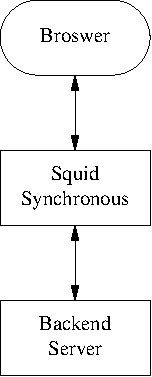
\includegraphics[width=.2\textwidth]{graph/reverse_squid.pdf}}\hspace{30pt}
  \subfloat[nginx代理模式]{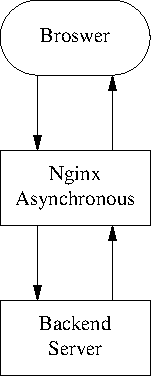
\includegraphics[width=.2\textwidth]{graph/reverse_nginx.pdf}}
  \caption{两种代理模式比较}
  \label{fig:squidVSnginx}
\end{figure}

squid同步传输:浏览器发起请求,而后请求会立刻被转到后台,于是在浏览器和
后台之间就建立了一个通道。在请求发起直到请求完成,这条通道都是一直存在
的。

nginx异步传输:浏览器发起请求,请求不会立刻转到后台,而是将请求数据(
header )先收到nginx上,然后nginx再把这个请求发到后端, 后端处理完之后把数
据返回到nginx上, nginx将数据流发到浏览器,这点和lighttpd有点不同,
lighttpd是将后端数据完全接收后才发送到浏览器。

那么这到底有什么好处呢?

\begin{enumerate}[itemsep=0pt,parsep=0pt]
\item 假设用户执行一个上传文件操作,因为用户网速又比较慢,因此需要花半
  个小时才能把文件传到服务器。squid的同步代理在用户开始上传后就和后台建
  立了连接,半小时后文件上传结束,由此可见,后台服务器连接保持了半个小
  时;而 nginx异步代理就是先将此文件收到nginx上,因此仅仅是nginx和用户
  保持了半小时连接,后台服务器在这半小时内没有为这个请求开启连接,半小
  时后用户上传结束,nginx才将上传内容发到后台,nginx和后台之间的带宽是
  很充裕的,所以只花了一秒钟就将请求发送到了后台,由此可见,后台服务器
  连接保持了一秒。同步传输花了后台服务器半个小时,异步传输只花一秒,可
  见优化程度很大。

\item 在上面这个例子中,假如后台服务器因为种种原因重启了,上传文件就自
  然中断了,这对用户来说是非常恼火的一件事情,想必我们也有上传文件传到
  一半被中断的经历。用nginx代理之后,后台服务器的重启对用户上传的影响减
  少到了极点,而nginx是非常稳定的并不需要常去重启它,即使需要重启,利用
  kill -HUP就可以做到不间断重启nginx。

\item 异步传输可以令负载均衡器更有保障,为什么这么说呢?在其它的均衡器
  ( lvs/haproxy/apache 等)里,每个请求都是只有一次机会的,假如用户发起
  一个请求,结果该请求分到的后台服务器刚好挂掉了,那么这个请求就失败了;
  而 nginx因为是异步的,所以这个请求可以重新发往下一个后台,下一个后台
  返回了正常的数据,于是这个请求就能成功了。还是用用户上传文件这个例子,
  假如不但用了nginx代理,而且用了负载均衡,nginx把上传文件发往其中一台
  后台,但这台服务器突然重启了,nginx收到错误后,会将这个上传文件发到另
  一台后台,于是用户就不用再花半小时上传一遍。

\item 假如用户上传一个10GB大小的文件,而后台服务器没有考虑到这个情况,
  那么后台服务器岂不要崩溃了。用nginx就可以把这些东西都拦在nginx上, 通
  过nginx的上传文件大小限制功能来限制,另外nginx性能非常有保障,就放心
  的让互联网上那些另类的用户和nginx对抗去吧。
\end{enumerate}

\subsection{Nginx 与 Lua 结合}

%%% Local Variables:
%%% mode: latex
%%% TeX-master: t
%%% End:


\chapter{LAMP}

\section{安装依赖包}

Needless to say, you should install required system packages. So you
cancontinue the next steps. :-)

Be sure these packages are installed:

\small{
\begin{verbatim}
  gcc
  gcc-c++
  flex
  bison
  autoconf
  automake
  bzip2-devel
  ncurses-devel
  libjpeg-devel
  libpng-devel
  libtiff-devel
  freetype-devel
  pam-devel
\end{verbatim}
}
\normalsize

\section{安装额外的包}

In this section, we need to compile and install four packages:

\begin{enumerate}[itemsep=0pt,parsep=0pt]
\item GD2
  \small{
\begin{verbatim}
  [root@lamp ~] # cd /usr/local/src
  [root@lamp src] # tar xzvf gd-2.0.34.tar.gz
  [root@lamp src] # cd gd-2.0.34
  [root@lamp gd-2.0.34] # ./configure --prefix=/usr/local/gd2
  [root@lamp gd-2.0.34] # make
  [root@lamp gd-2.0.34] # make install  
\end{verbatim}
  }
  \normalsize

\item LibXML2
  \small{
\begin{verbatim}
  [root@lamp ~] # cd /usr/local/src
  [root@lamp src] # tar xzvf libxml2-2.6.29.tar.gz
  [root@lamp src] # cd libxml2-2.6.29
  [root@lamp libxml2-2.6.29] # ./configure --prefix=/usr/local/libxml2
  [root@lamp libxml2-2.6.29] # make
  [root@lamp libxml2-2.6.29] # make install
\end{verbatim}
  }
  \normalsize

\item LibMcrypt
  \small{
\begin{verbatim}
  [root@lamp ~] # cd /usr/local/src
  [root@lamp src] # tar xjvf libmcrypt-2.5.8.tar.bz2
  [root@lamp src] # cd libmcrypt-2.5.8
  [root@lamp libmcrypt-2.5.8] # ./configure --prefix=/usr/local/libmcrypt
  [root@lamp libmcrypt-2.5.8] # make
  [root@lamp libmcrypt-2.5.8] # make install
\end{verbatim}
  }
  \normalsize

\item OpenSSL
  \small{
\begin{verbatim}
  [root@lamp ~] # cd /usr/local/src
  [root@lamp src] # tar xzvf openssl-0.9.8e.tar.gz
  [root@lamp src] # cd openssl-0.9.8e
  [root@lamp openssl-0.9.8e] # ./config --prefix=/usr/local/openssl
  [root@lamp openssl-0.9.8e] # make
  [root@lamp openssl-0.9.8e] # make test
  [root@lamp openssl-0.9.8e] # make install
\end{verbatim}
  }
  \normalsize

\end{enumerate}

\section{编译安装MySQL}

\small{
\begin{verbatim}
  [root@lamp ~] #tar xzvf mysql-5.0.27.tar.gz
  [root@lamp ~] # cd mysql-5.0.27
  [root@lamp mysql-5.0.27] # ./configure \
  "--prefix=/usr/local/mysql" \
  "--localstatedir=/var/lib/mysql" \
  "--with-mysqld-user=mysql" \
  "--without-debug" \
  "--with-big-tables" \
  "--with-extra-charsets=all" \
  "--with-pthread" \
  "--enable-static" \
  "--enable-thread-safe-client" \
  "--with-client-ldflags=-all-static" \
  "--with-mysqld-ldflags=-all-static" \
  "--enable-assembler" \
  "--without-isam" \
  "--without-innodb" \
  "--without-ndb-debug"
  
  [root@lamp msyql-5.0.27] # make
  [root@lamp mysql-5.0.27] # make install
  [root@lamp mysql-5.0.27] # useradd mysql
  [root@lamp mysql-5.0.27] # cd /usr/local/mysql
  [root@lamp mysql] # bin/mysql_install_db --user=mysql
  [root@lamp mysql] # chown -R root:mysql .
  [root@lamp mysql] # chown -R mysql /var/lib/mysql
  [root@lamp mysql] # cp share/mysql/my-huge.cnf /etc/my.cnf
  [root@lamp mysql] # cp share/mysql/mysql.server /etc/rc.d/init.d/mysqld
  [root@lamp mysql] # chmod 755 /etc/rc.d/init.d/mysqld
  [root@lamp mysql] # chkconfig --add mysqld
  [root@lamp mysql] # chkconfig --level 3 mysqld on
  [root@lamp mysql] # /etc/rc.d/init.d/mysqld start
  [root@lamp mysql] # bin/mysqladmin -u root password 'clear123'
\end{verbatim}
}
\normalsize

\section{编译安装Apache}

\small{
\begin{verbatim}
  [root@lamp src] # cd /usr/local/src
  [root@lamp src] # tar xjvf httpd-2.2.4.tar.bz2
  [root@lamp src] # cd httpd-2.2.4
  [root@lamp httpd-2.2.4] # ./configure \
  "--prefix=/usr/local/apache2" \
  "--with-included-apr" \
  "--enable-so" \
  "--enable-deflate=shared" \
  "--enable-expires=shared" \
  "--enable-rewrite=shared" \
  "--enable-static-support" \
  "--disable-userdir"
  [root@lamp httpd2.2.4] # make
  [root@lamp httpd2.2.4] # make install
  [root@lamp httpd2.2.4] # echo '/usr/local/apache2/bin/apachectl start' \
  > >> /etc/rc.local
\end{verbatim}
}
\normalsize

\section{编译安装PHP}

\small{
\begin{verbatim}
  [root@lamp ~] # cd /usr/local/src
  [root@lamp src] # tar xjvf php-5.2.3.tar.bz2
  [root@lamp php-5.2.3] # cd php-5.2.3
  [root@lamp php-5.2.3] # ./configure \
  "--prefix=/usr/local/php" \
  "--with-apxs2=/usr/local/apache2/bin/apxs" \
  "--with-config-file-path=/usr/local/php/etc" \
  "--with-mysql=/usr/local/mysql" \
  "--with-libxml-dir=/usr/local/libxml2" \
  "--with-gd=/usr/local/gd2" \
  "--with-jpeg-dir" \
  "--with-png-dir" \
  "--with-bz2" \
  "--with-freetype-dir" \
  "--with-iconv-dir" \
  "--with-zlib-dir " \
  "--with-openssl=/usr/local/openssl" \
  "--with-mcrypt=/usr/local/libmcrypt" \
  "--enable-soap" \
  "--enable-gd-native-ttf" \
  "--enable-memory-limit" \
  "--enable-ftp" \
  "--enable-mbstring" \
  "--enable-exif" \
  "--disable-ipv6" \
  "--disable-cgi" \
  "--disable-cli"
  [root@lamp php-5.2.3] # make
  [root@lamp php-5.2.3] # make install
  [root@lamp php-5.2.3] # mkdir /usr/local/php/etc
  [root@lamp php-5.2.3] # cp php.ini-dist /usr/local/php/etc/php.ini
\end{verbatim}
}
\normalsize

\section{安装Zend加速器}

\small{
\begin{verbatim}
  [root@lamp ~]# cd /usr/local/src
  [root@lamp ~]# tar xf ZendOptimizer-3.2.8-linux-glibc21-i386.tar.gz
  [root@lamp ~]# ./ZendOptimizer-3.2.8-linux-glibc21-i386/install.sh
\end{verbatim}
}
\normalsize

\section{整合Apache与PHP}

We should modify configure file httpd.conf:

\small{
\begin{verbatim}
[root@lamp ~]# emacs /usr/local/apache2/conf/httpd.conf
\end{verbatim}
}
\normalsize

Find this line,

\small{
\begin{verbatim}
AddType application/x-gzip .gz .tgz
\end{verbatim}
}
\normalsize

Add on line under this line,

\small{
\begin{verbatim}
AddType application/x-httpd-php .php
\end{verbatim}
}
\normalsize

Find these lines,

\small{
\begin{verbatim}
<IfModule dir_module>
DirectoryIndex index.html
<IfModule>
\end{verbatim}
}
\normalsize

Change them like this,

\small{
\begin{verbatim}
<IfModule dir_module>
DirectoryIndex index.html index.htm index.php
<IfModule>
\end{verbatim}
}
\normalsize

Find these lines and uncomment them,

\small{
\begin{verbatim}
#Include conf/extra/httpd-mpm.conf
#Include conf/extra/httpd-info.conf
#Include conf/extra/httpd-vhosts.conf
#Include conf/extra/httpd-default.conf
\end{verbatim}
}
\normalsize

When finished, save it! Then restart apache service,

\small{
\begin{verbatim}
[root@lamp ~]# /usr/local/apache2/bin/apachectl restart
\end{verbatim}
}
\normalsize

%%% Local Variables:
%%% mode: latex
%%% TeX-master: t
%%% End:


% \section{Nagios}
\label{sec:Nagios}

\subsection{关于Nagios}
\label{subsec:AboutNagios}

Nagios是一款非常优秀的监控软件。


\chapter{多网卡绑定bonding}

Linux bonding提供将多个网络接口设备捆绑为单个网络接口设置来使用,用于网
络负载均衡及网络冗余。

以太网平衡设备即使用两个或两个以上的网络接口模拟一个虚拟的网络接口用以
外部网络连接。这多个真实网络接口可以连接在同一交换设备或多个交换设备上,
以达到多通路高可用性。在所有真实网络接口中可以指定其中某些真实网络接口
活跃,其他真实网络接口在活跃的真实网络接口故障时接管网络传输;也可以指
定所有真实网络接口活跃,分担全部网络传输带宽。
 
通道绑定(Channel bonding)需要服务器至少拥有2个以太网卡,当使用绑定功能
的时候,bonding模块会使用第一个实际网卡的MAC地址来通信,在侦测到这个网
卡失败以后,它会把这个MAC地址指定到另一块网卡上。

\section{bonding的几种模式}

bonding只能提供链路监测,即从主机到交换机的链路是否接通。如果只是交换机
对外的链路down掉了,而交换机本身并没有故障,那么bonding会认为链路没有问
题而继续使用。
 
miimon是用来进行链路监测的。 比如:miimon=100,那么系统每100ms监测一次链
路连接状态,如果有一条线路不通就转入另一条线路;mode的值表示工作模式,
他共有0,1,2,3,4,5,6七种模式,作者遇到的场景是使用的1,0,6三种,
其他场景适合哪些模式作者也不清楚。
 
mode=1,表示fault-tolerance (active-backup)提供网络冗余功能,工作方式是
主备模式,也就是说默认情况下只有一块网卡工作,另一块做备份。
 
mode=0,表示load balancing (round-robin)为负载均衡模式,两块网卡都工作,
但是与网卡相连的交换机必须做特殊配置( 这两个端口应该采取聚合方式),因
为做bonding的这两块网卡是使用同一个MAC地址。
 
mode=6,表示load balancing (round-robin)为负载均衡方式,两块网卡都工作,
但是该模式下无需配置交换机,因为做bonding的这两块网卡是使用不同的MAC地
址。
 
\section{RHEL下配置bonding}

华为RH1288服务器共有8块网卡,eth0与eth1做bond0,对应管理网
段172.16.25.X,主备模式;eth2与eth3做bond1,此网段暂没有配置IP信息,主
备模式;eth4与eth5做bond2,对应存储网段10.10.2.X,主备模式。

编辑/etc/modprobe.d/dist.conf文件,在文件末尾添加如下几行,开
启bonding功能\footnote{这是RHEL6U4的系统,如果是RHEL5系列的机器,配置文
  件则为/etc/modprobe.conf}。

\begin{verbatim}
# vim /etc/modprobe.d/dist.conf
alias bond0 bonding
options bond0 mode=1 miimon=100

alias bond1 bonding
options bond1 mode=1 miimon=100

alias bond2 bonding
options bond2 mode=1 miimon=100
\end{verbatim}

编辑虚拟网络接口配置文件bond0,

\begin{verbatim}
# vim /etc/sysconfig/network-scripts/ifcfg-bond0
DEVICE=bond0
ONBOOT=yes
BOOTPROTO=none
NETWORK=
IPADDR=
NETMASK=
GATEWAY=
USERCTL=no
\end{verbatim}

分别编辑eth0与eth1网络接口文件ifcfg-eth0与ifcfg-eth1,

\begin{verbatim}
# vim /etc/sysconfig/network-scripts/ifcfg-eth0
DEVICE=eth0
BOOTPROTO=none
TYPE=Ethernet
ONBOOT=yes
USERCTL=no
MASTER=bond0 
SLAVE=yes

# vim /etc/sysconfig/network-scripts/ifcfg-eth1
DEVICE=eth1
BOOTPROTO=none
TYPE=Ethernet
ONBOOT=yes
USERCTL=no
MASTER=bond0 
SLAVE=yes
\end{verbatim}

由于该机器对应的交换机接口为VLAN 210,所以,需要在bond0接口上配置VLAN。

\begin{verbatim}
# vconfig add bond0 210
\end{verbatim}

这样就产生了一个bond0.210的虚拟网络接口,这样就可以启用该接口,并配
置IP信息,

\begin{verbatim}
# ifconfig bond0.210 up
# vim /etc/sysconfig/network-scripts/ifcfg-bond0.210
DEVICE=bond0.210
BOOTPROTO=none
ONBOOT=yes
USERCTL=no
IPADDR=172.16.25.93
NETMASK=255.255.255.0
GATEWAY=172.16.25.254
VLAN=yes
\end{verbatim}

查看上面已配置的VLAN信息,

\begin{verbatim}
# cat /proc/net/vlan/config
VLAN Dev name	 | VLAN ID
Name-Type: VLAN_NAME_TYPE_RAW_PLUS_VID_NO_PAD
bond0.210      | 210  | bond0

# cat /proc/net/vlan/bond0.210 
bond0.210  VID: 210	 REORDER_HDR: 1  dev->priv_flags: 1
         total frames received         4663
          total bytes received       224809
      Broadcast/Multicast Rcvd          38

      total frames transmitted          228
       total bytes transmitted         44140
            total headroom inc           0
           total encap on xmit            0
Device: bond0
INGRESS priority mappings: 0:0  1:0  2:0  3:0  4:0  5:0  6:0 7:0
EGRESS priority mappings:
\end{verbatim}

\section{SuSE下配置bonding}

bond0配置:

\begin{verbatim}
# cat /etc/sysconfig/network/ifcfg-bond0
DEVICE='bond0'
ONBOOT='yes'
BOOTPROTO='static'
IPADDR='0.0.0.0/24'   
STARTMODE='auto'
BONDING_MASTER='yes'
BONDING_MODULE_OPTS='mode=1 miimon=100'
BONDING_SLAVE0='eth0'
BONDING_SLAVE1='eth1'
USERCONTROL='no'
\end{verbatim}

br0配置:

\begin{verbatim}
# cat /etc/sysconfig/network/ifcfg-br0
BOOTPROTO='static'
BRIDGE='yes'
BRIDGE_FORWARDDELAY='0'
BRIDGE_PORTS='bond1'
BRIDGE_STP='off'
IPADDR='0.0.0.0/24'    	##管理网ip
STARTMODE='auto'
USERCONTROL='no'

# cat /etc/sysconfig/network/ifcfg-vlan0     ##为网卡打Vlan Tag
BOOTPROTO='static'
ETHERDEVICE='br0'
IPADDR='145.240.21.11/24'
STARTMODE='auto'
USERCONTROL='no'
VLAN_ID='210'                       ##上联核心交换机端口的Vlan号

# cat /proc/net/vlan/config         ##验证Vlan是否设置成功
VLAN Dev name | VLAN ID
Name-Type: VLAN_NAME_TYPE_RAW_PLUS_VID_NO_PAD
vlan0         | 210 | br0
\end{verbatim}

\section{单网卡多IP配置}
\label{sec:SingleCardMultiIP}

% \chapter{LVM硬盘管理及扩容}

% LVM是 Logical Volume Manager(逻辑卷管理)的简写,它由Heinz Mauelshagen在
% Linux 2.4内核上实现。LVM将一个或多个硬盘的分区在逻辑上集合,相当于一个
% 大硬盘来使用,当硬盘的空间不够使用的时候,可以继续将其它的硬盘的分区加
% 入其 中,这样可以实现磁盘空间的动态管理,相对于普通的磁盘分区有很大的灵
% 活性。
 
% 与传统的磁盘与分区相比,LVM为计算机提供了更高层次的 磁盘存储。它使系统
% 管理员可以更方便的为应用与用户分配存储空间。在LVM管理下的存储卷可以按需
% 要随时改变大小与移除(可能需对文件系统工具进行升 级)。LVM也允许按用户组
% 对存储卷进行管理,允许管理员用更直观的名称(如"sales'、 'development')代
% 替物理磁盘名(如'sda'、'sdb')来标识存储卷。
 
% 如图所示LVM模型:
 
% 由四个磁盘分区可以组成一个很大的空间,然后在这些空间上划分一些逻辑分区,
% 当一个逻辑分区的空间不够用的时候,可以从剩余空间上划分一些空间给空间不
% 够用的分区使用。

% \chapter{使用U盘安装Gnu系统}

% 使用U盘安装系统在某些时候还是很方便的,其安装速度也是蛮给力的。为什么会
% 有本章内容呢?主要是小白在装机中发现有的机器不带光驱,而且身边也没有移
% 动光驱可用,并且也不能从网络启动来安装系统。由于这些诸多限制,小白就想
% 可不可以使用U盘安装呢?网上搜索了一下,果然可以,而且安装速度比光驱快!
% 下面就介绍一下如何使用U盘来安装Gnu/Linux系统。

% \section{准备工作}

% \begin{enumerate}[itemsep=0pt,parsep=0pt]
% \item 4G以上的优盘,格式化成FAT32
% \item 镜像编辑软件UltraISO
% \item Gnu/Linux镜像文件
% \end{enumerate}

% \section{制作启动盘}

% \begin{enumerate}[itemsep=0pt,parsep=0pt]
% \item 启动软件后打开Linux ISO文件
% \item 点击“工具”,“加载到虚拟光驱”,点击“加载”
% \item 打开“我的电脑”找到虚拟光驱的盘符 
% \item 找到“boot.ISO”文件,双击打开
% \item 点击“启动”,“写入硬盘镜像”
% \item 选择你的U盘,写入方式:USB-HDD+,点击“写入”,开始写入引导文件到
%   U盘
% \item 等待一会儿,消息栏提示“刻录成功”,引导文件写入完毕
% \item 确认是否写入成功和盘符是否选对:打开“我的电脑”,可移动存储栏里
%   出现 以:“Red Hat Ent”命名的盘符,代表写入成功
% \end{enumerate}

% \section{开始安装Gnu/Linux}

% 在安装过程中,需要选择Grub安装位置时,需要注意一下,我们要把Grub安装到
% 系统盘中,默认是安装在U盘里的,这时可以修改之以继续安装。如果这一步没有
% 修改,也没有关系,等系统安装完毕重启时,不要拔掉U盘。一切就绪进入系统后,
% 可以使用grub-install命令重新安装Grub到指定的盘中。

\chapter{RAID技术}

RAID技术有各种级别之分,包括RAID0、RAID1、RAID2、RAID3、RAID4、RAID5、
RAID5E、RAID5EE、RAID6、RAID10等。作者接触最多的是RAID0、RAID1、RAID5及
RAID10这些RAID级别,其他级别在实际工作当中并没有见到,这里就不在介绍。

\section{RAID基础知识}

RAID最初是1987年在加利福尼亚大学进行的一个科研项目,后来由伯克利分校的
D.A. Patterson教授在1988年正式提出。

RAID是Redundant Array of Inexpensive Disks的缩写,直译为“廉价冗余磁盘阵
列”,最初是为了组合多块小容量的廉价磁盘来代替大容量的昂贵磁盘,同时希望
在磁盘失效时不会对数据造成影响而开发出的一种磁盘存储技术。

后来随着磁盘研发技术的不断提升,硬盘容量越来越大,成本却不断下降,所以
RAID中“Inexpensive(廉价)”一词已经失去意义,于是将这个词用
“Independent(独立)”来替代,RAID就成了”独立冗余磁盘阵列“,也简称为”磁
盘阵列“,但这只是名称的变化,实质性的内容并没有改变。

\subsection{RAID解决了什么问题}

通俗地说,RAID就是通过将多个磁盘按照一定的形式和方案组织起来,通过这样
的形式能够获取比单个磁盘更高的速度、更好的稳定性、更大的存储能力的存储
解决方案,我们不必关心磁盘阵列究竟由多少块磁盘组成,使用中整个整列就如
同一块磁盘一样。所以,RAID技术能够为计算机系统提供以下三个方面的优异性
能:

\begin{enumerate}[itemsep=0pt,parsep=0pt]
\item 提供更大的存储空间
\begin{quote}
  使用RAID技术,就可以把多块磁盘组成一个更大的存储空间供我们使用。比如,
  利用RAID0技术把5块1TB的硬盘组织起来,能够提供5TB的存储空间。
\end{quote}

\item 提供更快的传输速度
\begin{quote}
  著名的摩尔定律告诉我们,CPU的性能每隔18个月就会提高一倍,可见其速度增
  长之快。然而,机械硬盘作为计算机中最重要的存储设备,在容量飞速增长的
  同时,速度却提高缓慢,已经成为计算机速度发展的瓶颈。

  如果采用RAID技术,可以让很多机械硬盘同时传输数据,而这些硬盘在逻辑上
  又表现为一块硬盘,所以使用RAID可以达到单个磁盘几倍、甚至N多倍的速率。
  也就是说,RAID技术可以通过在多个磁盘上同时存储和读取数据的方式来大幅
  提高存储系统的数据吞吐量。
\end{quote}

\item 提高更高的安全性
\begin{quote}
RAID可以通过数据校验提供容错功能,在很多RAID模式中都有较为完备的冗余措
施,甚至是直接相互的镜像备份,从而大大提高来RAID系统的容错性,让系统的
稳定性更好、安全性更高。
\end{quote}
\end{enumerate}

\section{RAID实现方式}

\subsection{RAID0数据组织原理}

RAID0是无冗余、无校验的磁盘阵列,实现RAID0,至少需要两个以上硬盘,它将
两个以上的硬盘合并成一块,数据同时分散在每块磁盘中,因为带宽加倍,所以
读写速度加倍,RAID0的理论速度是单块硬盘的N倍,但是由于数据并不是保存在
一个硬盘上,而是分成数据块保存在不同的硬盘上,所以安全性也下降N倍,只要
任何一块磁盘损坏就会丢失所有数据。

RAID0是最简单的一种RAID形式,目的是把多块物理盘连接在一起形成一个容量更
大的存储设备,RAID0逻辑盘的容量等于物理盘的容量乘以成员盘的数目。

原理图

RAID0只是单纯地提高读写性能,并没有数据的可靠性提供保证,而且其中的任何
一个物理盘失效都将影响到所有数据。因此,RAID0不能用于数据安全性要求高的
场合。
\subsection{RAID1数据组织原理}

RAID1通过磁盘数据镜像实现数据的冗余,在两块磁盘上产生互为备份的数据,当
其中一块成员盘出现故障时,系统还可以从另外一块成员盘中读取数据。因此,
RAID1可以提供更好的冗余性。

RAID1又称为磁盘镜像,需要在两个物理盘共同构建,使用磁盘镜像技术,方法是
在工作磁盘之外再加一额外的备份磁盘,两个磁盘所存储的数据完全一样,数据
写入工作磁盘的同时亦写入备份磁盘,也就是将一块物理盘的内容完全复制到另
一块物理盘上。所以,两块物理盘所构成的RAID1阵列,其容量仅等于一块磁盘的
容量,其数据分布情况如图所示。

原理图

RAID1是磁盘阵列中单位成本最高的,但提供来很高的数据安全性和可用性。当一
个物理盘失效时,系统可以自动切换到镜像盘上读写,而不需要重组失效的数据。

RAID1是所有RAID等级中实现成本最高的一种,尽管如此,我们还是选择RAID1来
保存那些关键性的重要数据。

\subsection{RAID10数据组织原理}

\subsection{RAID5数据组织原理}

\section{MegaRAID Cli工具基本使用}
\label{sec:MegaraidCmd}

我们都是使用过LSI的Web界面去配置RAID,虽听起来很高大上,但整个配置过程
是那么的令人蛋疼。配置完成后,我们还要按“Ctrl+Alt+Del”组合键来重启机
器,步骤虽有些繁琐,但仍能令人接受。MegaRAID Cli工具是在命令行模式下操
作RAID控制器的,它的优点之一就是做完RAID之后,可以直接使用并不需要重
启操作系统,而且操作简单方便。

写这一节的目的并不是推荐使用该工具,而是熟悉了原来的配置界面,不愿意再
学新的东西。若不是同事的提示,还不知有这种很xx的工具,使用起来确实很酷,
愿意跟大家分享一下使用过程。

要想使用该工具,首先系统上要安装相应的软件包,这里省略安装过程。安装完
毕之后,工具默认会安装在/opt/MegaRAID/MegaCli的目录下。

本次使用该命令行工具的场景:新到了两块Intel的SATA接口400GB的SSD硬盘,欲
测其性能。原来的服务器上自带了4块600GB的磁盘并做了RAID10,这四块磁盘分
别占据了第0、1、2、3这四个硬盘插槽,在第4、第5个插槽放置了SSD盘,操作系
统使用的是SLES 11.2。下面是具体的操作过程,

\subsection{制作RAID}

\begin{enumerate}[itemsep=0pt,parsep=0pt]
\item 查看RAID卡的设备号
\begin{verbatim}
# cd /opt/MegaRAID/MegaCli
# ./MegaCli64 -PDList -aAll |grep "Device ID"
Enclosure Device ID: 252
Enclosure Device ID: 252 
Enclosure Device ID: 252
Enclosure Device ID: 252
Enclosure Device ID: 252
Enclosure Device ID: 252
\end{verbatim}

说明:上面的输出,表示我们有一个RAID卡,因为这些ID是一样的。这个卡下面
有6个盘,这里的ID号需要记下来,后面做RAID时需要用到。可以把该RAID的ID号
理解为主设备号。
	
\item 查看Slot ID以确认有无错序的情况
\begin{verbatim}
# ./MegaCli64 -PDList -aAll |grep "Slot"  
Slot Number: 0
Slot Number: 1
Slot Number: 2
Slot Number: 3
Slot Number: 4
Slot Number: 5
\end{verbatim}

说明:这里的Slot Number号需要记下来,后面做RAID时需要用到。可以吧该
Slot的ID理解为次设备号。
	
\item 查看Foreign信息
\begin{verbatim}
# ./MegaCli64 -PDList -aAll |grep "Foreign State"
Foreign State: None
Foreign State: None 
Foreign State: None
Foreign State: None
Foreign State: Foreign 
Foreign State: Foreign 
\end{verbatim}

说明:状态显示为“Foreign”的磁盘,说明是新添加进来的或者是未使用的。这
两个为“Foreign”状态的正是我们新添加的SSD盘。接下来的操作就是清除这些
“Foreign”状态的盘。
	
\item 清除盘的Foreign信息
\begin{verbatim}
# ./MegaCli64 -CfgForeign -Clear -a0
\end{verbatim}
	
\item 新做RAID,在Slot4和Slot5上做RAID0
\begin{verbatim}
# ./MegaCli64 -CfgLdAdd -r0 [252:4,252:5] WT Direct -a0
\end{verbatim}
\end{enumerate}

说明:如果做RAID1,只需要把r0改为r1即可。

\subsection{删除RAID}

当测试完毕RAID0级别的SSD盘时,要开始测试RAID1级别下Intel SATA SSD的性能。
所以,之前制作的RAID0要被删除了。在删除之前,我们需要知道被删除的
Target Id,然后方可删除该组RAID。

查看有多少个RAID级别,找到我们想要删除的Target Id,其中“Target Id:n”,
n即为第n组RAID。

\begin{verbatim}
# ./MegaCli64 -LdInfo -Lall -aALL 
\end{verbatim}

删除阵列,
\begin{verbatim}
# ./MegaCli64 -CfgLdDel -L1 -a0
\end{verbatim}
	
附录:名词解释
磁盘缓存策略:
\begin{verbatim}
WT(Write Through)
WB(Write Back)
NORA(NO Read Ahead)
RA(Read Ahead)
ADRA(Adaptive Read Ahead)
\end{verbatim}

